\documentclass[a4j,  9pt]{ltjsarticle}

\usepackage{../mypackage}

\begin{document}

  \section{集合論}
    数学でモデルを扱うとき集合論的に思考すると上手にそのモデルを扱うことができる。これは数学の問題を解く場合も同様である。では集合論とは何か, 概要を確認しておこう。
    %\begin{multicols}{2} %*を用いれば真ん中の直線を最初から最大にできる

    \subsection{集合の定義}
      集合とはその名の通り, いくつかのものをひとまとめにして考えた\textbf{ものの集まりのこと}である。
      特に集合論では\textbf{もの}のことを要素という。\par
      またある集合$\ds A$は他の集合$\ds B$と共通部分を持ったり, はたまたその集合$\ds A$自体が他の集合$\ds B$の一部分となるケースも考えられる。
      そのような場合順に\textbf{$\ds AとB$の共通部分}, \textbf{$\ds AはBの$部分集合}という。

      \begin{center}
        \begin{tikzpicture}[auto]
        
          %Ven diagram1
          \def \circleRadius{1}
          \def \leftCirclePoint{(0,  0)}
          \def \rightCirclePoint{(1,  0)}
          \def \centerPointOfShareArea{(0.5,  0)}
          \def \leftCircleNamePoint{(0,  1)}
          \def \rightCircleNamePoint{(1,  1)}

          %Ven diagram2
          \def \circleARadius{0.7}
          \def \circleBRadius{1}
          \def \circleAPoint{(4,  -0.2)}
          \def \circleBPoint{(4,  0)}
          \def \circleANamePoint{(4,  \circleARadius-0.2)}
          \def \circleBNamePoint{(4,  \circleBRadius)}

          \scope
            %Aのベン図
            \clip \leftCirclePoint circle (\circleRadius);
            \fill [fill=white] \rightCirclePoint circle (\circleRadius);
          \endscope

          \scope
            %Bのベン図
            \clip \rightCirclePoint circle (\circleRadius);
            \fill [pattern=north west lines] \leftCirclePoint circle (\circleRadius);
          \endscope

          \draw \leftCirclePoint circle (\circleRadius);
          \draw \rightCirclePoint circle (\circleRadius);
          \node[set label,  text=black] (A) at \leftCircleNamePoint {$\ds A$};
          \node[set label,  text=black] (B) at \rightCircleNamePoint {$\ds B$};

          %共通部分ラベル
          \draw[semithick,  -,  stealth] \centerPointOfShareArea--(0.5,  -1.5);
          \draw[semithick,  -,  stealth] (0.5,  -1.5)--(-1,  -1.5);
          \node[set label,  text=black] (CAP) at (-1,  -1.5) {$\ds AとBの共通部分$};


          \fill[pattern=north west lines] \circleAPoint circle (\circleARadius);
          \draw                           \circleAPoint circle (\circleARadius);
          \draw                           \circleBPoint circle (\circleBRadius);
          \node[set label,  text=black] (A') at \circleANamePoint {$\ds A$};
          \node[set label,  text=black] (B') at \circleBNamePoint {$\ds B$};

        \end{tikzpicture}
      \end{center}

      また, 上図のように集合を視覚的に図式化したものを\textbf{ベン図}という。

      \subsubsection{集合の例}
        例として「原子」という集合を考えてみよう。(ここでいう原子は量子論・化学における, 物質を構成する原子を指すものとする)\par
        原子には様々な種類があり, 例えば水素原子\ce{_{1}H}や酸素原子\ce{_{8}O}などがある。
        このとき\ce{_{1}H}や\ce{_{8}O}は原子集合の要素であるといえる。\par
        またさらに水素元素\ce{H}や酸素元素\ce{O}はそれぞれ水素原子\ce{_{1}H}の全同位体を含んだ集合, 酸素原子\ce{_{8}O}の全同位体を含んだ集合ゆえ原子集合の部分集合である。

    \subsection{集合論の記号}
      ここまでは言葉を用いて集合について少し論じた。しかしいちいち言葉で説明するのは少々面倒であり, しかも読みづらい。そこで記号を導入してみよう。

      \subsubsection{基本的な記法}
        例えば$\ds A$という集合を自然数$\ds 1 \thicksim 5$を要素に持つ集合として定義したい場合$\ds A \define \{ 1,  2,  3,  4,  5 \}$と書く。
        つまり要素を$\ds \{\}$で囲むことでそれらを要素に持つという意味を表すのである。
        この記法を\textbf{\ruby{外延的記法}{がい|えん|てき|き|ほう}}という。\par
        ついでこの場合$\ds 1$は$\ds A$の要素であるから, これを$\ds 1 \in A$と書く。\par
        
        %強制的に改段
        %\columnbreak
        
        また, 同じ意味の定義で\par
        $\ds A \define \{ n \in \mathbb{N} \mid 1 \leq n \leq 5 \}$と表すこともできる。
        この場合は具体的に要素を書き出すことをせずに, \par
        $\ds \{ n \in ($母体となる集合$\ds ) \mid n$が満たす条件$\ds \}$といった具合に条件を満たすもので集合を定義する記法である。
        この記法は\textbf{\ruby{内包的記法}{ない|ほう|てき|き|ほう}}という。

        \paragraph{内包的記法の例}
          例えば次のように偶数全体の集合として$\ds A$を定義してみる。\par
          \begin{equation*}
            \begin{split}
              $\ds A \define \{ n \in \mathbb{Z} \mid \exists_{m \in \mathbb{Z}} [n = 2m] \}$\\
            \end{split}
          \end{equation*}
          このように存在記号や全称記号を用いた条件で定義されることはよくあるしとても簡潔でわかりやすい。

          \footnote{
            他の例として次のようなものがある\par
            開区間 $\ds (a,  b) \define \{ x \in \mathbb{R} \mid a < x < b \}$, 
            閉区間 $\ds [a,  b] \define \{ x \in \mathbb{R} \mid a \leq x \leq b \}$
          }

      \blank

      \footnote{
        要素を持たない集合を空集合という。
      }

    \columnbreak

    \subsection{論理学との関連}
      先に見たように集合を定義する際に, 内包的記法で論理記号を用いて表現することができる。
      これについて論理学的な観点から見てみよう。\par

      \subsubsection{条件の真理集合}
        例として, $\ds x \in \mathbb{R}$についての条件$\ds p(x)$があるとき, この$\ds p(x)$が真となるような$\ds x$の集合を$\ds P$としよう。
        つまり集合$\ds P$は次のように定義される。

        \begin{equation*}
          \begin{split}
            $\ds P \define \{ x \in \mathbb{R} \mid p(x) \}$
          \end{split}
        \end{equation*}

        またベン図は以下。

        \begin{center}
          \begin{tikzpicture}[auto]

            %Rのベン図
            \draw[line](0,  0)rectangle(120pt,  80pt);
            \node[set label,  text=black] at (10pt,  80pt) {$\ds \mathbb{R}$}

            %Pのベン図
            \fill[pattern=north west lines,  draw=black] (60pt,  40pt) ellipse (20pt);
            \node[set label, text=black] at (60pt,  60pt) {$\ds P$};

          \end{tikzpicture}
        \end{center}

        このように, 条件$\ds p(x)$に対しこれを真にしうる$\ds x$の集合$\ds P$のことを, 条件$\ds p(x)$の\textbf{真理集合}という。\par
        これにより, 抽象的でやや複雑な論理関係も集合論に関係付けることでベン図等を用いて視覚化することもできるので, 真理集合を用いることは論理関係の理解の助けになる。
        
        また最初に見た偶数全体の集合$\ds A$は, $\ds n \in \mathbb{Z}$についての条件$\ds \exists_{m \in \mathbb{Z}} [n = 2m]$の真理集合と言える。

      \subsubsection{論理演算子と集合の演算子}
        全体集合を$\ds U$とするとき, $\ds x \in U$に関する条件$\ds p(x),  q(x)$があるとし, これらに関する真理集合をそれぞれ$\ds P,  Q$としよう。
        このとき集合$\ds U,  P,  Q$の包含関係は条件$\ds p(x),  q(x)$の論理関係に依存する。\par

        例えば$\ds p(x) \land q(x)$を満たす$\ds x \in U$が存在する場合, ベン図は以下のように描ける。

        \begin{center}
          \begin{tikzpicture}[auto]

            %Uのベン図
            \draw[line](0,  0)rectangle(120pt,  80pt);
            \node[set label,  text=black] at (10pt,  80pt) {$\ds U$}

            \def \circleRadius{20pt}
            \def \leftCirclePoint{(50pt,  40pt)}
            \def \rightCirclePoint{(70pt,  40pt)}
            \def \centerPointOfShareArea{(60pt,  40pt)}
            \def \leftCircleNamePoint{(50pt,  60pt)}
            \def \rightCircleNamePoint{(70pt,  60pt)}

            \scope
              %Pのベン図
              \clip \leftCirclePoint circle (\circleRadius);
              \fill [fill=white] \rightCirclePoint circle (\circleRadius);
            \endscope

            \scope
              %Qのベン図
              \clip \rightCirclePoint circle (\circleRadius);
              \fill [pattern=north west lines] \leftCirclePoint circle (\circleRadius);
            \endscope

            \draw \leftCirclePoint circle (\circleRadius);
            \draw \rightCirclePoint circle (\circleRadius);
            \node[set label,  text=black] (P) at \leftCircleNamePoint {$\ds P$};
            \node[set label,  text=black] (Q) at \rightCircleNamePoint {$\ds Q$};

            %共通部分ラベル
            \draw[semithick,  -,  stealth] \centerPointOfShareArea--(60pt,  -10pt);
            \node[set label,  text=black] (CAP) at (60pt,  -10pt) {$\ds p(x) \land q(x)$の真理集合};

          \end{tikzpicture}
        \end{center}

        すなわち, ($\ds p(x) \land q(x)$の真理集合) $\ds = \{ x \in U \mid p(x) \land q(x) \}= P \cap Q$であることがわかり, 
        $\ds \land$を$\ds \cap$とした実質的な論理演算子の分配則が成立しているように見える。\par
        これ以外のベン図もまとめると以下である。

        \begin{center}
          \begin{tikzpicture}[auto]

            \def \circleRadius{20pt}

            %%%%%%%%%%% FIRST %%%%%%%%%%%
            \def \firstURadius{(120pt,  80pt)}
            \def \firstUPoint{(0,  0)}
            \def \firstULabelPoint{(10pt,  80pt)}
            \def \firstPCirclePoint{(60pt,  40pt)}
            \def \firstPLabelPoint{(60pt,  60pt)}
            \def \firstLogicPanelPoint{(60pt,  -10pt)}

            %Uのベン図
            \scope
              \fill[pattern=north west lines] \firstUPoint rectangle (\firstURadius);
              \draw[line] \firstUPoint rectangle (\firstURadius);
            \endscope
            \node[set label,  text=black] at \firstULabelPoint {$\ds U$}

            %Pのベン図
            \scope
              \clip \firstPCirclePoint circle (\circleRadius);
              \fill [fill=white] \firstPCirclePoint circle (\circleRadius);
              \draw [line] \firstPCirclePoint circle (\circleRadius);
            \endscope
            \node[set label,  text=black] at \firstPLabelPoint {$\ds P$};

            %論理ラベル
            \node[set label,  text=black] at \firstLogicPanelPoint {$\ds \{ x \in U \mid \overline{p(x)} \} = \overline{P}$};
            %%%%%%%%%%% FIRST %%%%%%%%%%%

            %%%%%%%%%%% SECOND %%%%%%%%%%%
            \def \secondURadius{(280pt,  80pt)}
            \def \secondUPoint{(160pt,  0)}
            \def \secondULabelPoint{(170pt,  80pt)}
            \def \secondPCirclePoint{(210pt,  40pt)}
            \def \secondPLabelPoint{(210pt,  60pt)}
            \def \secondQCirclePoint{(230pt,  40pt)}
            \def \secondQLabelPoint{(230pt,  60pt)}
            \def \secondLogicPanelPoint{(220pt,  -10pt)}
            
            %Uのベン図
            \scope
              \draw[line] \secondUPoint rectangle (\secondURadius);
            \endscope
            \node[set label,  text=black] at \secondULabelPoint {$\ds U$}

            %Pのベン図
            \scope
              \clip \secondPCirclePoint circle (\circleRadius);
              \fill [pattern=north west lines] \secondPCirclePoint circle (\circleRadius);
              \draw [line] \secondPCirclePoint circle (\circleRadius);
            \endscope
            \node[set label,  text=black] at \secondPLabelPoint {$\ds P$};

            %Qのベン図
            \scope
              \clip \secondQCirclePoint circle (\circleRadius);
              \fill [pattern=north west lines] \secondQCirclePoint circle (\circleRadius);
              \draw [line] \secondQCirclePoint circle (\circleRadius);
            \endscope
            \node[set label,  text=black] at \secondQLabelPoint {$\ds Q$};

            %論理ラベル
            \node[set label,  text=black] at \secondLogicPanelPoint {$\ds \{ x \in U \mid p(x) \lor q(x) \} = P \cup Q$};
            %%%%%%%%%%% SECOND %%%%%%%%%%%

            %%%%%%%%%%% THIRD %%%%%%%%%%%
            \def \thirdURadius{(120pt,  -110pt)}
            \def \thirdUPoint{(0,  -30pt)}
            \def \thirdULabelPoint{(10pt,  -30pt)}
            \def \thirdPCirclePoint{(50pt,  -70pt)}
            \def \thirdPLabelPoint{(50pt,  -50pt)}
            \def \thirdQCirclePoint{(70pt,  -70pt)}
            \def \thirdQLabelPoint{(70pt,  -50pt)}
            \def \thirdLogicPanelPoint{(140pt,  -120pt)}

            %Uのベン図
            \scope
              \fill[pattern=north west lines] \thirdUPoint rectangle (\thirdURadius);
              \draw[line] \thirdUPoint rectangle (\thirdURadius);
            \endscope
            \node[set label,  text=black] at \thirdULabelPoint {$\ds U$}

            %Pのベン図
            \scope
              \clip \thirdPCirclePoint circle (\circleRadius);
              \fill [fill=white] \thirdPCirclePoint circle (\circleRadius);
              \draw [line] \thirdPCirclePoint circle (\circleRadius);
            \endscope
            \node[set label,  text=black] at \thirdPLabelPoint {$\ds P$};

            %Qのベン図
            \scope
              \clip \thirdQCirclePoint circle (\circleRadius);
              \fill [pattern=north west lines] \thirdQCirclePoint circle (\circleRadius);
              \draw [line] \thirdQCirclePoint circle (\circleRadius);
            \endscope
            \node[set label,  text=black] at \thirdQLabelPoint {$\ds Q$};

            %論理ラベル
            \node[set label,  text=black] at \thirdLogicPanelPoint {$\ds \{ x \in U \mid p(x) \Longrightarrow q(x) \} = \overline{P} \cup Q \quad (\because ならば文の基礎定理)$};
            %%%%%%%%%%% THIRD %%%%%%%%%%%

            %%%%%%%%%%% FOURTH %%%%%%%%%%%
            \def \fourthURadius{(280pt,  -110pt)}
            \def \fourthUPoint{(160pt,  -30pt)}
            \def \fourthULabelPoint{(170pt,  -30pt)}
            \def \fourthQCirclePoint{(220pt,  -70pt)}
            \def \fourthQLabelPoint{(220pt,  -40pt)}
            \def \fourthPCirclePoint{(220pt,  -70pt)}
            \def \fourthPLabelPoint{(220pt,  -55pt)}

            %Uのベン図
            \scope
              \fill[pattern=north west lines] \fourthUPoint rectangle (\fourthURadius);
              \draw[line] \fourthUPoint rectangle (\fourthURadius);
            \endscope
            \node[set label,  text=black] at \fourthULabelPoint {$\ds U$}

            %Qのベン図
            \scope
              \clip \fourthQCirclePoint circle (\circleRadius);
              \fill [pattern=north west lines] \fourthQCirclePoint circle (30pt);
            \endscope
            \draw [line] \fourthQCirclePoint circle (30pt);
            \node[set label,  text=black] at \fourthQLabelPoint {$\ds Q$};

            %Pのベン図
            \scope
              \clip \fourthPCirclePoint circle (\circleRadius);
              \fill [pattern=north west lines] \fourthPCirclePoint circle (15pt);
              \draw [line] \fourthPCirclePoint circle (15pt);
            \endscope
            \node[set label,  text=black] at \fourthPLabelPoint {$\ds P$};
            %%%%%%%%%%% FOURTH %%%%%%%%%%%

          \end{tikzpicture}
        \end{center}

    \subsection{集合同士の積}
      実数に積という演算があるのと同じように集合間にも積の演算がある。それを\textbf{直積}, または\textbf{デカルト積}という。ここではそれについてみておこう。\par

      \subsubsection{直積の定義}
        $\ds A, B \ne \varnothing$なる集合に対し, それらの要素$\ds a \in A,  b \in B$を対にとった集合$\ds (a,  b)$を直積と定義する。
        この対には\textbf{順序}があるため特に\textbf{順序対}という。
        式で定義すれば以下。\par
        
        \begin{equation*}
          \begin{split}
            $\ds A \times B \define \{ (a,  b) \mid a \in A,  b \in B \}$\\
          \end{split}
        \end{equation*}

        直積は\textbf{それぞれの要素を対にとった集合}として定義されているので, この演算には一般に交換法則が成立しないことがわかる。

        \footnote{
          直積をとる集合の片方または両者が空集合の場合順序対の作りようがないためその結果は空集合として定義されている。\par
          $\ds A = \varnothing \lor B = \varnothing$のとき$\ds A \times B \define \varnothing$
        }
        
        \paragraph{交換法則が成立しない一つの例}
          \begin{equation*}
            \begin{split}
              &$\ds A \define \{ a,  b,  c \}$\\
              &$\ds B \define \{ 1,  2 \}$
            \end{split}
          \end{equation*}

          とする。$\ds A$と$\ds B$の直積$\ds A \times B$を計算してみよう。\par
          例えば$\ds a \in A,  1 \in B$であるから求めるべき直積には積の順と同順の順序対$\ds (a,  1)$が要素として存在する。\par
          では逆に$\ds B \times A$の場合は$\ds (1,  a)$が要素として存在する。しかしこの場合$\ds (a,  1)$は要素として存在しない。
          順序対は対の順序を考慮するから$\ds (a,  1) \ne (1,  a)$である。\par
          ゆえに$\ds A \times B = B \times A$はこの場合成り立たない。\par

        \vspace{9pt}\\

        以上のように一般に直積は$\ds A \times B \ne B \times A$である。\par
        しかし, 特例としてこれが成立する場合もある。その例は次のような場合である。

        \paragraph{交換法則が成立する特例}

          \begin{equation*}
            \begin{split}
              $\ds A,  B \define \{ 1,  2\}$\\
            \end{split}
          \end{equation*}

          とする。ここで$\ds A \times B$を考えてみると

          \begin{equation*}
            \begin{split}
              $\ds 1 \in A,  1 \in B$\\
            \end{split}
          \end{equation*}

          であるから考えている直積には順序対$\ds (1,  1)$が要素として存在する。\par
          実際にすべて書き出してみると\par

          \begin{equation*}
            \begin{split}
              $\ds A \times B = \{ (1,  1),  (1,  2),  (2,  1),  (2,  2) \}$\\
            \end{split}
          \end{equation*}

          となっている。もしこれをひっくり返したとしても結果は同じである。\par
          よってこの場合$\ds A \times B = B \times A$が成立する。\par

        \vspace{9pt}\\

        この場合なぜ交換法則が成立するのか考えてみると, 直積をとった集合同士が全く同じ要素を持つ集合同士であったことが要因であることがわかる。\par
        (また, 自身で直積をとった場合$\ds A \times A = A^2$と表し, 一般に$\ds n$回直積をとった時$\ds A^n$と表す。)\par
        ゆえにこれを一般化すると次のように言える。(ただし有限集合の場合に限る)\par

        \begin{eqnarray}
          \begin{split}
            $\ds ( A = \varnothing \lor B = \varnothing \lor A = B ) \Longleftrightarrow $&$\ds A \times B = B \times A$ \label{eq:ex-cartesian-product}
          \end{split}
        \end{eqnarray}

        これは対偶をとってもわかる通り直積に持っていてほしい特性が論理的に正しく保持されていることも確認できる。\par

        \begin{equation*}
          \begin{split}
            \eqref{eq:ex-cartesian-product}
            $\ds \Longleftrightarrow " A \times B \ne B \times A \Longleftrightarrow ( A \ne \varnothing \land B \ne \varnothing \land A \ne B ) "$\\
          \end{split}
        \end{equation*}

      \subsubsection{直積の要素の個数(濃度)}
        直積の要素の個数はどのように求まるか, 先ほどの積の交換法則が成立しない例の状況で考えてみよう。\par
        このとき$\ds A \times B$を計算してみると

        \begin{equation*}
          \begin{split}
            $\ds A \times B = \{ (a,  1),  (a,  2),  (b,  1),  (b,  2),  (c,  1),  (c,  2) \}$\\
          \end{split}
        \end{equation*}

        直積の要素は「順序対」であったからこの場合の要素数は$\ds 6$である。\par
        これを一般の集合(有限集合のとき)の場合にも適用できるように考えてみよう。次のように表にしてみるとわかりやすいだろう。

        \vspace{9pt}\\

        \begin{center}
          \begin{tablehere}
            \centering
            \label{tab:hogehoge}
            \begin{tabular}{c|ccc}
                    & $\ds a$       & $\ds b$       & $\ds c$     \\ \hline
                1   & $\ds (a,  1)$  & $\ds (b,  1)$  & $\ds (c,  1)$\\
                2   & $\ds (a,  2)$  & $\ds (b,  2)$  & $\ds (c,  2)$\\
            \end{tabular}
          \end{tablehere}
        \end{center}

        \vspace{9pt}\\

        つまり要素数はこの表で順序対が作る長方形の面積のようなものと対応していることがわかる。\par
        よって一般に
        
        \begin{equation*}
          \begin{split}
            $\ds | A \times B | = | A | \times | B |$\\
          \end{split}
        \end{equation*}

        と表せることがわかる。(ただし有限集合同士の直積の場合のみ)

    \columnbreak

    \subsection{実数平面や実数空間の表現}
      実数全体の集合$\ds \mathbb{R}$は他の視点から見ると実数の数直線を表す集合と考えられる。\par
      では実数平面や実数空間などは集合を使ってどのように表せるだろうか。
      ここで次のような直積を考えてみる。

      \begin{equation*}
        \begin{split}
          $\ds \mathbb{R} \times \mathbb{R} = \mathbb{R}^2$
        \end{split}
      \end{equation*}

      これは幾何的に解釈すると, 実数の数直線同士を平行でない向きに並べたときにできる平面のすべての点を要素に持つ集合である。
      それはまさに実数平面のことである。

      \begin{center}
        \begin{tikzpicture}

          \coordinate[label=below  left:O] (O) at (0, 0); %原点O
          \coordinate (XS) at (-1, 0); %x軸最小
          \coordinate (XL) at (1, 0); %x軸最大
          \coordinate (YS) at (0, -1); %y軸最小
          \coordinate (YL) at (0, 1); %y軸最大
          \draw[semithick, ->, >=stealth] (XS)--(XL) node[right] {$\mathbb{R}$}; %x軸
          \draw[semithick, ->, >=stealth] (YS)--(YL) node[above] {$\mathbb{R}$}; %y軸

        \end{tikzpicture}
      \end{center}
      
      このことを意識して直積を書き直すと

      \begin{equation*}
        \begin{split}
          $\ds \mathbb{R}^2 = \{ (x,  y) \mid x \in \mathbb{R},  y \in \mathbb{R} \}$
        \end{split}
      \end{equation*}

      と書ける。\par

      \vspace{9pt}\\

      同様の議論で実数空間($\ds 3$次元空間)も次のような直積で表せる。

      \begin{equation*}
        \begin{split}
          $\ds \mathbb{R}^3 = \{ (x,  y,  z) \mid x \in \mathbb{R},  y \in \mathbb{R},  z \in \mathbb{R} \}$
        \end{split}
      \end{equation*}

      \begin{center}
        \begin{figurehere}
          \centering
          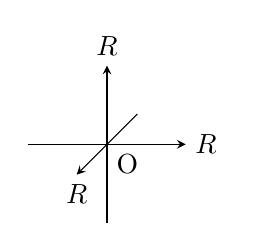
\begin{tikzpicture}

            \draw[-stealth](-1, 0, 0) -- (1, 0, 0) node[right]{$\mathbb{R}$};
            
            \draw[-stealth](0, -1, 0) -- (0, 1, 0) node[above]{$\mathbb{R}$};
            
            \draw[-stealth](0, 0, -1) -- (0, 0, 1) node[below]{$\mathbb{R}$};
            
            \draw (0, 0, 0) node[below right]{O};
          
          \end{tikzpicture}
        \end{figurehere}
      \end{center}

      これを用いれば直積の交換法則が不成立な理由も次のように考えて直観的に理解できる。\par

      \subsubsection{幾何的に直積の交換法則が不成立であることを確認してみる}
        ある点$\ds (a,  b)$を考えてみよう。(ただし$\ds a \ne b$とする。)\par
        二次元平面上では$\ds a \ne b$ならば$\ds (a,  b) \ne (b,  a)$である。\par
        これは順序対が反転すると幾何的に異なる量へ変化するためである。

        \begin{center}
          \begin{tikzpicture}
          
            \coordinate[label=below  left:O] (O) at (0, 0); %原点O
            \coordinate (XS) at (-0.5, 0); %x軸最小
            \coordinate (XL) at (3, 0); %x軸最大
            \coordinate (YS) at (0, -0.5); %y軸最小
            \coordinate (YL) at (0, 3); %y軸最大
            \draw[semithick, ->, >=stealth] (XS)--(XL) node[right] {$x$}; %x軸
            \draw[semithick, ->, >=stealth] (YS)--(YL) node[above] {$y$}; %y軸
            
            % (a,  b)
            \coordinate (P1) at (2, 1.5); %右頂点
            \fill (P1) circle (0.05); %点の塗りつぶし
            \node (x) at (2.2,  1.7) {$\ds (a,  b)$};%座標の可視化
            
            % (b,  a)
            \coordinate (P2) at (1.5, 2); %右頂点
            \fill (P2) circle (0.05); %点の塗りつぶし
            \node (x) at (1.7,  2.2) {$\ds (b,  a)$};%座標の可視化
            
            \draw[dashed] ($(XS)!(P1)!(XL)$)node[below]{$\ds a$}--(P1)--($(YS)!(P1)!(YL)$)node[left]{$\ds b$};
            \draw[dashed] ($(XS)!(P2)!(XL)$)node[below]{$\ds b$}--(P2)--($(YS)!(P2)!(YL)$)node[left]{$\ds a$};
              %右頂点から各軸への垂線

          \end{tikzpicture}
        \end{center}

        すなわちこれは幾何的に順序対が異なるものであることを説明しており, 直積の順序で順序対が変化することが異なる量へ変化していることの根拠である。\par
        実際このことは直積(特に順序対)の定義であった。
        それに対しこの幾何的説明は, 順序対が対の順序を考慮することの合理性を示していると考えられる。

      \subsection{参考: ユークリッド空間}
        先ほど$\ds \mathbb{R}$の直積を積み立てることで$\ds 2,  3$次元空間を集合で表現することができた。
        ではここでこれの一般化をしてみよう。\par
        次のように$\ds N \in \mathbb{N}$個の直積を考えてみる。

        \begin{equation*}
          \begin{split}
            $\ds \mathbb{R}^N = \{ (x_1,  x_2,  \cdots ,  x_N) \mid x_1 \in \mathbb{R},  x_2 \in \mathbb{R},  \cdots ,  x_N \in \mathbb{R} \}$
          \end{split}
        \end{equation*}

        % \[
        %   \left(
        %     \begin{tabular}{l}
        %       または次のようにも表せる。\\
        %       \begin{equation*}
        %         \begin{split}
        %           $\ds \mathbb{R}^3 = \{ (x,  y,  z) \mid x \in \mathbb{R},  y \in \mathbb{R},  z \in \mathbb{R} \}$\\
        %         \end{split}
        %       \end{equation*}
        %     \end{tabular}
        %   \right)
        % \]
        
        ここに得られた集合$\ds \mathbb{R}^N$をユークリッド空間という。\par
        つまり任意の$\ds N \in \mathbb{N}$に対して呼ぶので$\ds \mathbb{R}^2$の$\ds 2$次元平面や$\ds \mathbb{R}^3$の$\ds 3$次元空間もユークリッド空間である。
    
    \subsection{実数集合の最大値・最小値}
      より一般的の高い最大値・最小値についての議論をするには, 複素解析的に議論をする必要があり内容が少々ハードである。
      ここでは少し範囲を絞り, 実数集合の場合について議論することにする。\par
      
      \vspace{9pt}\\

      実数空間$\ds \mathbb{R}$上には「大小関係 $\ds \leq$」と呼ばれる二項関係が定義されており, これは全順序としての性質

      \begin{numcases}
        $\ds \forall_{x \in \mathbb{R}} [ x \leq x]$ & \label{ax:inequality-to-real-1} \\
        $\ds \forall_{x,  y \in \mathbb{R}} [ (x \leq y \land y \leq x) \Rightarrow x = y ]$ & \label{ax:inequality-to-real-2} \\
        $\ds \forall_{x,  y,  z \in \mathbb{R}} [ (x \leq y \land y \leq z) \Rightarrow x \leq z ]$ & \label{ax:inequality-to-real-3} \\
        $\ds \forall_{x,  y \in \mathbb{R}} [ x \leq y \lor y \leq x ]$ & \label{ax:inequality-to-real-4}
      \end{numcases}

      \vspace{9pt}\\

      を満たすことを公理として定める。\par

      この下で, 次のものを定義する。

      \begin{breakbox}
        任意の$\ds x,  y \in \mathbb{R}$に対し, 
        \begin{equation*}
          \begin{split}
            $\ds x < y \defineProposition (x \leq y \land x \ne y)$
          \end{split}
        \end{equation*}
      \end{breakbox}

      また, 実数空間$\ds \mathbb{R}$の空でない部分集合$\ds A$があるとき, ある$\ds a \in A$が任意の$\ds x \in A$以上であるとき, この$\ds a$を$\ds A$の最大値(最大元)とよぶ。\par
      つまり

      \begin{equation*}
        \begin{split}
          $\ds \max A = a \defineProposition \forall_{x \in A} [ x \leq a ]$
        \end{split}
      \end{equation*}

      \footnote{
        定義に「以下 $\ds \leq$」を用いる理由は, 任意の$\ds x \in A$としているため$\ds x = a$の場合もあるので, それを考慮しているためである。
      }

      次に, 同様の状況$\ds A \subset \mathbb{R} \land A \ne \varnothing$において, ある$\ds a \in A$が任意の$\ds x \in A$以下であるとき, この$\ds a$を$\ds A$の最小値(最小元)とよぶ。\par
      つまり

      \begin{equation*}
        \begin{split}
          $\ds \min A = a \defineProposition \forall_{x \in A} [ a \leq x ]$
        \end{split}
      \end{equation*}

      \footnote{
        今紹介したもの以外の話や詳しい議論は以下を参照\par
        https://wiis.info/math/real-number/definition-of-real-number/magnitude-relation/\par
        https://wiis.info/math/real-number/definition-of-real-number/maximu-value-and-minimum-value/
      }

    \subsection{実数集合の有界性}
      $\ds A \subset \mathbb{R}$なる$\ds A$に対し$\ds M \in \mathbb{R}$が

      \begin{equation*}
        \begin{split}
          $\ds \forall_{x \in A} [ x \leq M ]$
        \end{split}
      \end{equation*}
      
      と取れるとき, \textbf{$\ds A$は上に有界である}という。
      少し範囲を広くして言えば, $\ds A (\subset \mathbb{R})$が最大値を持つならば$\ds A$は上に有界であるといえる。
      ここに注意として, "$\ds A$が最大値をもつことは$\ds A$が上に有界であることと同値ではない"である。\par

      同様にこれの"下バージョン"について, 同様の状況$\ds A \subset \mathbb{R}$なる$\ds A$に対し$\ds m \in \mathbb{R}$が

      \begin{equation*}
        \begin{split}
          $\ds \forall_{x \in A} [ x \geq m ]$
        \end{split}
      \end{equation*}

      と取れるとき, \textbf{$\ds A$は下に有界である}という。
      これも少し範囲を広くして言えば, $\ds A (\subset \mathh{R})$が最小値を持つならば$\ds A$は下に有界であるといえる。
      これも先ほどと同様の注意を払おう。\par

      ではなぜ同値ではないのか。次のような具体例を見てみよう。\par

      例えば$\ds A = \{ x \in \mathbb{R} \mid x > m \}$であるとき, もちろん

      \begin{equation*}
        \begin{split}
          $\ds \forall_{x \in A} [ x > m ]$
        \end{split}
      \end{equation*}

      であり, $\ds m$は$\ds A$の最小値ではないし, そもそも$\ds A$は最小値をもたない。したがってこのような場合の表現が難しいために先ほどの議論をしたのであった。
      \footnote{
        $\ds A = \{ x \in \mathbb{R} \mid x > m \}$ならば$\ds m \notin A$であるから, このようなとき$\ds m$は$\ds A$の最小値ではない。
      }
      
    \subsection{上限と下限}

      ここで, 有界な集合に対するその上・下の集合を考える。\par
      
      上に有界な$\ds A (\subset \mathbb{R})$に対し

      \begin{equation*}
        \begin{split}
          $\ds S$ & $\ds \define \{ y \in \mathbb{R} \mid \forall_{x \in A} [ y \geq x ] \}$
        \end{split}
      \end{equation*}

      と定義して, このような$\ds S$を\textbf{$\ds A$の上界}と言い, この上界の最小値$\ds \min S$を\textbf{$\ds A$の上限}と言い$\ds \sup A$と書く。

      \vspace{9pt}\\

      同様に下に有界な$\ds A (\subset \mathbb{R})$に対し

      \begin{equation*}
        \begin{split}
          $\ds I$ & $\ds \define \{ y \in \mathbb{R} \mid \forall_{x \in A} [ y \leq x ] \}$
        \end{split}
      \end{equation*}

      と定義して, このような$\ds I$を\textbf{$\ds A$の下界}と言い, この下界の最大値$\ds \max I$を\textbf{$\ds A$の下限}と言い$\ds \inf A$と書く。\par

      \vspace{9pt}\\

      今定義した$\ds \sup A,  \inf A$はそれぞれ$\ds \max A,  \min A$の拡張となっていることがわかり, 
      任意の$\ds A (\subset \mathbb{R})$は$\ds \max A,  \min A$が存在するとは言えなかったことに対して$\ds \sup A,  \inf A$は必ず存在することがわかる。-

    \newpage

    \subsection{写像}
      集合間を関係付ける概念として写像がある。ここではこの写像についてみていこう。
      
      \subsubsection{写像の定義}
        $\ds X,  Y$を空でない集合とする。\par
        任意の$\ds x \in X$に対し, ある$\ds y \in Y$が一意に定まるとき, このような\textbf{対応規則}$\ds f$を\textbf{$\ds X$から$\ds Y$への写像$\ds f$}と呼び, 
        $\ds f:X \mapsto Y$や, 各集合の任意の要素を強調した場合には$\ds f(x) = y$と書く。\par
        また, $\ds X$の要素$\ds x$を写像$\ds f$によって写した$\ds Y$の要素が$\ds y$であることを, \textbf{$\ds x$を写像$\ds f$によって移した像}といい, この場合の$\ds x$を\textbf{原像}という。\par
        このことを強調して記す場合には, $\ds x \stackrel{f}{\mapsto} y$のように書く。
        \footnote{
          \textbf{$\ds X,  Y$が数を要素とする集合}の場合特に\textbf{関数}と呼ぶ。
        }

        \begin{center}
          \begin{tikzpicture}[auto]
          
            %Xのベン図
            \fill[color=black!50!white,  draw=black] (0, 0) ellipse (20pt and 40pt);
            \node[set label, text=black] at (0,  40pt) {$\ds X$};

            %Yのベン図
            \draw (80pt, 0) ellipse (20pt and 40pt);
            \fill[color=black!50!white,  draw=black] (80pt,  0) ellipse (10pt and 20pt); % black!50!white で黒と白50%
            \node[set label, text=black] at (80pt,  40pt) {$\ds Y$};
            \node[set label, text=black] at (80pt,  20pt) {$\ds R_f$};

            %写像f
            \draw[->] (0,  0) to node {$\scriptstyle f$} (80pt,  0);

          \end{tikzpicture}
        \end{center}

        したがって, 写像$\ds f$は次のように定義される。

        \begin{equation*}
          \begin{split}
            $\ds f:X \mapsto Y \defineProposition \forall_{x \in X} [\exists!_{y \in Y} [y = f(x)]]$
          \end{split}
        \end{equation*}

        \paragraph{定義域・値域}
          写像$\ds f: X \mapsto Y$について, $\ds X$を$\ds f$の\textbf{定義域}と呼び, 
          また, $\ds x \in X$を写像$\ds f$によって写した像である$\ds y \in Y$の集合を$\ds f$の\textbf{値域}と呼ぶ。
          \footnote{
            文面上では勘違いしやすいが, 一般には$\ds R_f = Y$ではなく$\ds R_f \subset Y$である。
          }\par
          すなわち$\ds f$の値域$\ds R_f$とは, 「$\ds x \in X \land y = f(x)$を満たす$\ds x$が存在する」ような$\ds y$の集合であるから, 厳密に次のように定義される。
          
          \begin{center}
            \begin{equation*}
              \begin{split}
              $\ds R_f \define \{ y \in Y \mid \exists_x[ x \in X \land y = f(x) ] \}$
              \end{split}
            \end{equation*}
          \end{center}
        
      \subsubsection{単射と全射}
        写像$\ds f: X \mapsto Y$があるとする。\par
        \paragraph{単射}
          ここに「任意の$\ds X$の異なる要素$\ds x, x'$について, それぞれを写像$\ds f$で写した像$\ds y, y'$が異なる」とき, 
          写像$\ds f$を特に\textbf{単射}であるといい, ないしは\textbf{一対一の写像}ともいう。
          \footnote{
            紛らわしいが, 「一対一の写像」は「一対一対応」ではない。なぜなら, 単射であるからと言って必ずしも$\ds 値域 = Y$ではないため, 任意の$\ds y \in Y$に逆像が存在するとは言えないためである。
          }\par
          このような場合, 写像$\ds f$が単射であることを強調して$\ds f: X \hookrightarrow Y$とかくことがある。\par

          \begin{center}
            \begin{tikzpicture}[auto]
            
              %Xのベン図
              \fill[color=black!50!white,  draw=black] (0, 0) ellipse (20pt and 40pt);
              \node[set label,  text=black] (X) at (0,  40pt) {$\ds X$};

              %Yのベン図
              \draw (80pt, 0) ellipse (20pt and 40pt);
              \fill[color=black!50!white,  draw=black] (80pt,  0) ellipse (10pt and 20pt); % black!50!white で黒と白50%
              \node[set label,  text=black] (Y) at (80pt,  40pt) {$\ds Y$};

              %x->y
              \node (x) at (0,  15pt) {$\ds x$};
              \node (y) at (80pt,  15pt) {$\ds y$};
              \draw[->] (0,  10pt) to node {$\scriptstyle f(x)$} (80pt,  10pt);

              %x'->y'
              \node (x') at (0,  -3pt) {$\ds x'$};
              \node (y') at (80pt,  -3pt) {$\ds y'$};
              \draw[->] (0,  -10pt) to node {$\scriptstyle f(x')$} (80pt,  -10pt);

            \end{tikzpicture}
          \end{center}

          つまり, 写像$\ds f$が単射であるための条件は, 

          \begin{center}
            \begin{equation*}
              \begin{split}
                
                &$\ds x \neq x' \Longrightarrow f(x) \neq f(x')$\\
  
              \end{split}
            \end{equation*}
          \end{center}

          である。
          あるいは対偶をとることにより

          \begin{center}
            \begin{equation*}
              \begin{split}
                
                &$\ds f(x) = f(x') \Longrightarrow x = x'$\\
  
              \end{split}
            \end{equation*}
          \end{center}
          と考えてもよい。\par
          したがって, 写像$\ds f$が単射であることは次のように定義される。

          \begin{center}
            \begin{equation*}
              \begin{split}
                &$\ds f:X \hookrightarrow Y \defineProposition \forall_{x, x' \in X} [x \neq x' \Longrightarrow f(x) \neq f(x')]$\\
              \end{split}
            \end{equation*}
          \end{center}

          \footnote{
            単射の定義について, $\ds f$が写像であることを前提としない場合, 写像であることの定義も含めて次のように表せる
            $\ds f:X \hookrightarrow Y \Longleftrightarrow \forall_{x \in X} [\exists!_{y \in Y} [y = f(x)] \land \forall_{x' \in X} [x \neq x' \Longrightarrow f(x) \neq f(x')] ]$
          }

        \blank

        \paragraph{全射}
          次に, 「任意の$\ds y \in Y$に対し, それが$\ds x \in X$を写像$\ds f$で写した像であるような$\ds x$が少なくとも一つ存在する」とき, 
          言い換えれば「任意の$\ds y \in Y$に対し, $\ds y = f(x)$となるような$\ds x \in X$が存在する」とき, 
          写像$\ds f$を特に\textbf{全射}であるという。\par
          この場合は, 写像$\ds f$が全射であることを強調して$\ds f: X \twoheadrightarrow Y$とかくことがある。\par

          \begin{center}
            \begin{tikzpicture}[auto]
            
              %Xのベン図
              \draw (0, 0) ellipse (20pt and 40pt);
              \fill[color=black!50!white,  draw=black] (0,  0) ellipse (10pt and 20pt); % black!50!white で黒と白50%
              \node[set label,  text=black] (X) at (0,  40pt) {$\ds X$};

              %Yのベン図
              \fill[color=black!50!white,  draw=black] (80pt, 0) ellipse (20pt and 40pt);
              \node[set label,  text=black] (Y) at (80pt,  40pt) {$\ds Y$};

              %x->y
              \node (x) at (0,  15pt) {$\ds x$};
              \node (y) at (80pt,  15pt) {$\ds y$};

              %x'->y'
              \node (x') at (0,  5pt) {$\ds x'$};
              \node (y') at (80pt,  -3pt) {$\ds y'$};

              %x''->y'
              \node (x'') at (0,  -7pt) {$\ds x''$};

              \draw[->] (0,  10pt) to node {$\scriptstyle f(x)$} (80pt,  10pt);
              \draw[->] (0,  0) to node {$\scriptstyle f(x')$} (80pt,  -10pt);
              \draw[->] (0,  -10pt) to node {} (80pt,  -10pt);
              \node[text=black] at (40pt,  -15pt) {$\scriptstyle f(x'')$}

            \end{tikzpicture}
          \end{center}

          したがって, 写像$\ds f$が全射であることは次のように定義される。

          \begin{center}
            \begin{equation*}
              \begin{split}
                &$\ds f:X \twoheadrightarrow Y \defineProposition \forall_{y \in Y} [ \exists_{x \in X} [ y = f(x) ] ]$\\
              \end{split}
            \end{equation*}
          \end{center}

      \subsubsection{全単射(一対一対応)}
        単射かつ全射であるような写像を, \textbf{全単射}という。
        つまり$\ds f: X \mapsto Y$が全単射であるとは, 「任意の$\ds y \in Y$に対して, $\ds f(x) = y$を満たす$\ds x \in X$がただ一つ存在する」ことである。
        すなわち, 単射と全射の合成写像である。(合成写像については後に述べることにする)

        \begin{center}
          \begin{tikzpicture}[auto]
          
            %Xのベン図
            \fill[color=black!50!white,  draw=black] (0, 0) ellipse (20pt and 40pt);
            \node[set label,  text=black] (X) at (0,  40pt) {$\ds X$};

            %Yのベン図
            \fill[color=black!50!white,  draw=black] (80pt, 0) ellipse (20pt and 40pt);
            \node[set label,  text=black] (Y) at (80pt,  40pt) {$\ds Y$};

            %x->y
            \node (x) at (0,  15pt) {$\ds x$};
            \node (y) at (80pt,  15pt) {$\ds y$};
            \draw[->] (0,  10pt) to node {$\scriptstyle f(x)$} (80pt,  10pt);

            %x'->y'
            \node (x') at (0,  -3pt) {$\ds x'$};
            \node (y') at (80pt,  -3pt) {$\ds y'$};
            \draw[->] (0,  -10pt) to node {$\scriptstyle f(x')$} (80pt,  -10pt);

          \end{tikzpicture}
        \end{center}

        したがって, 写像$\ds f$が全単射であることは次のように表せる。

        \begin{center}
          \begin{equation*}
            \begin{split}

              $\ds f: X \mapsto Y$が全単射である $\ds \Longleftrightarrow \forall_{y \in Y} [ \exists!_{x \in X} [ y = f(x) ] ]$

            \end{split}
          \end{equation*}
        \end{center}

        つまりは, 全射の定義における存在記号$\ds \exists$を唯一存在記号$\ds \exists!$に置き換えたもので, これが逆方向の一意性を示していることがわかる。
        これにより, 任意の$\ds x \in X$を$\ds f$によって写した像を$\ds y \in Y$とするとき, $\ds x$と$\ds y$が一対一に対応するのである。\par
        ところで, 任意の$\ds y \in Y$について$\ds y = f(x)$を満たす$\ds x \in X$がただ一つ存在するからと言って, 
        逆に任意の$\ds x \in X$について$\ds y = f(x)$を満たす$\ds y \in Y$の唯一存在について言及していないために
        「本当に$\ds \forall_{y \in Y} [ \exists!_{x \in X} [ y = f(x) ] ]$の成立が$\ds f: X \mapsto Y$が全単射であることと等価なのであろうか？」
        と疑問を持つかもしれないが, そもそも写像の定義として任意の$\ds x \in X$に対する$\ds y = f(x)$を満たす$\ds y \in Y$の唯一存在性が主張されているのでこれは自明と言ってよいのである。\par

        \paragraph{全単射の特徴}
          全単射の最初に挙げるべき特徴として, 
          
          \begin{center}
            \begin{equation*}
              \begin{split}
              
                \textbf{全単射である} $\ds \Longleftrightarrow$ \textbf{逆写像が存在する}
                
              \end{split}
            \end{equation*}
          \end{center}

          という事実である。
          これについては, 逆写像について論じる際に述べることにするのでそちらを参照されたい。

\end{document}